\documentclass[a4paper,12pt]{article} 
% Paquetes......................................................................
\usepackage{amsmath, amssymb, amsfonts, latexsym}
\usepackage[utf8]{inputenc}
\usepackage[T1]{fontenc}
\usepackage{palatino}
\usepackage[full]{textcomp}
\usepackage{hyperref}
\usepackage{eurosym}
\usepackage[makeroom]{cancel}
\usepackage{array}
\usepackage{pdfpages}
\usepackage{float} % para que las figuras no floten
\usepackage{subcaption}
\usepackage{soul} % para el highlight \hl
\usepackage{pdfpages} % para pegar otro pdf dentro de este

\textheight = 24 cm
\textwidth = 17 cm

\renewcommand{\arraystretch}{1.25}
\renewcommand{\contentsname}{Contenidos}


% INICIO DEL DOCUMENTO --------------------------------------------------------
\begin{document}
	
	\setlength{\parindent}{0.5cm}
	\setlength{\voffset}{-2cm}
	\setlength{\hoffset}{-2cm}
	
	\input{./include/portada.tex}
	
	\tableofcontents
	
\newpage

	\section{Introducción}
	% Introduction. High level overview of the ontology you plan to develop and brief description of the datasets and web pages that you plan to use.
		
	En el contexto de la iniciativa OpenCityData \cite{opencitydata} y del proyecto
Ciudades Abiertas \cite{ciudadesabiertas} se han desarrollado un buen número de
ontologías que permitan representar datos abiertos de ciudades, en muy diversas áreas (transporte,
gestión económica, equipamientos, servicios, etc.). Dentro de esta iniciativa se encuentran
muchas áreas todavía por desarrollar, y es una de ellas en las que se enmarca el desarrollo de
este trabajo.
	
	El objetivo es diseñar e implementar una ontología que represente de manera adecuada
instalaciones deportivas, sus características y acciones relacionadas. Las ontologías y otras
fuentes de conocimiento utilizadas durante el desarrollo de este trabajo serán citadas, y se puede
acceder a ellas a través de los hipervínculos de la bibliografía.
La ontología por desarrollar constituirá un modelo para representar los datos asociados a una
instalación deportiva, donde se entiende como instalación deportiva un recinto o construcción provista de los medios necesarios para la práctica, aprendizaje y competición de uno o más
deportes, y que está asociada, organizada y mantenida por una determinada organización. Como
iremos describiendo en los siguientes apartados de la memoria, se especificarán todos los
requisitos necesarios para la creación de la ontología, y se detallarán todas las características de
esta.
	
	A la hora de la creación de la ontología se han seguido las pautas que marca la metodología NeOn,
haciendo uso tanto de recursos ontológicos como no ontológicos para su reutilización y
reingeniería. Cada una de las actividades de la metodología ha sido realizada según la secuencia
especificada y con un planteamiento ordenado. Tras ello, se ha usado la herramienta Protégé para
la formalización en OWL de la ontología, OOPS! para su evaluación y WIDOCO para su documentación.
	
	\section{Metodología NeOn}
	% Make a short overview of the NeOn methodology making explicit:
	%   a. which scenarios you plan to follow
	%   b. which activities from the glossary of activities you plan to execute in your ontology development project
	
	La Metodología NeOn para la construcción de redes de ontologías es una metodología basada en
escenarios que se apoya en los aspectos de colaboración de desarrollo de ontologías y la
reutilización, así como en la evolución dinámica de las redes de ontologías en entornos
distribuidos
\cite{oeg-neon}.
	
	Como define esta metodología, hay un conjunto de nueve escenarios para la construcción de
ontologías, haciendo hincapié en la reutilización de recursos ontológicos, la reingeniería y la
fusión. Para este trabajo se han seguido los
siguientes escenarios:
	\begin{itemize}
		\item \textbf{Escenario 2: La reutilización y reingeniería de recursos no ontológicos (NOR).}
		Se llevan a cabo procesos de reutilización NOR para decidir, en base a los requisitos definidos, qué recursos no ontológicos se utilizarán para construir la red de la ontología. Posteriormente estos NOR se readaptarán mediante reingeniería.
		\item \textbf{Escenario 4: La reutilización y reingeniería de los recursos ontológicos.}
		Se llevan a cabo procesos de reutilización de recursos y se reorganizan los recursos ontológicos.
		\item \textbf{Escenario 7: Reutilización de los patrones de diseño de ontologías (ODPs).}
		\hl{Los desarrolladores de ontolog}ías acceden a repositorios de reutilización ODPs.
		\item \textbf{Escenario 9: Localización de recursos ontológicos.}
		\hl{Los desarrolladores de ontolog}ías adaptan una ontología a otras lenguas y la cultura las comunidades, obteniendo así una ontología multilingüe.
	\end{itemize}
	
	Otro punto importante dentro de la metodología NeOn es el glosario de actividades \cite{oeg-glossary}. Durante todo el proceso de construcción de
	nuestra ontología se han realizado actividades incluidas en este glosario. A continuación se listan
	algunas de las más importantes:
	
	\begin{itemize}
		\item \textbf{Ontology Requirements Specification.} Planteamiento de preguntas y la resolución de
		estas para detectar las necesidades y requisitos de la ontología.
		\item \textbf{Ontology Aligning.} Buscamos entre los diferentes recursos ontológicos los elementos comunes para evaluar qué recursos son más adecuados para nuestra ontología.
		\item \textbf{Ontology Annotation.} Se han asignado etiquetas (labels) y comentarios para enriquecer la ontología.
		\item \textbf{Ontology Comparison.} Al buscar ontologías ya creadas sobre el mismo dominio, se compararon y evaluaron  las diferencias entre ellas para elegir las ontologías más adecuadas para la reutilización.
		\item \textbf{Ontology Conceptualization.} Durante el proceso de adquisición, se organizó
		toda la información recopilada para crear un modelo conceptual que cubriese los
		requisitos definidos.
		\item \textbf{Control.} Se siguió la planificación temporal prevista para completar las tareas de
		desarrollo programadas.
		\item \textbf{Ontology Design Pattern Reuse.} Se han reusaron patrones de diseño para esta
ontología, concretamente el patrón de Normas y el de Servicios.
		\item \textbf{Ontology Diagnosis.} Gracias al uso de herramientas como OOPS! se pudieron evaluar los
fallos de la ontología y corregirlos durante el proceso de desarrollo.
		\item \textbf{Ontology Elicitation.} Se realizó una adquisición de estructuras conceptuales, como el T-Box, a partir de documentos de expertos del dominio de las instalaciones deportivas.
		\item \textbf{Ontology Erichment.} Extendiendo el número de relaciones y clases de algunas de las ontologías reutilizadas se logró completarlas y cubrir ciertos requisitos.
		\item \textbf{Ontology Implementation.} Una vez diseñado el modelo conceptual se transformó la ontología a un modelo formal (código OWL) gracias a Protégé.
		\item \textbf{Ontology Localization.} Las entidades y relaciones creadas se etiquetaron tanto en español
como en inglés.
		\item \textbf{Ontology Merging.} Se fusionaron clases y funciones de distintas ontologías para crear
una ontología nueva.
		\item \textbf{Ontology Search.} Se realizó una búsqueda de ontologías o módulos de ontologías
candidatas a ser reutilizadas.
		\item \textbf{Ontology Module Extraction.} Se extrajeron módulos concretos de ciertas ontologías.
		\item \textbf{Ontology Module Reuse.} Se reutilizaron los módulos extraídos de otras ontologías.
		\item \textbf{Non-Ontological Resource Reengineering.} Se reestructuraron recursos no
ontológicos para adaptarlos a la ontología.
		\item \textbf{Non-Ontological Resource Reuse.} Se reusaron recursos no ontológicos para
transformarlos en partes de la ontología.
		\item \textbf{Scheduling.} Se realizó una planificación de las actividades anteriores para
completarlas en el orden correcto dentro del plazo de entrega y así llevar un control de las mismas.
	\end{itemize}
	
	\section{Especificación de la ontología}
	% Ontology specification. You should include a complete ontology specification requirement document using the template explained during the lectures. The goal of the ontology should be clear enough. The document should include relevant competency questions and their answers.
	
	\subsection{Propósito}
	El objetivo de esta ontología se enmarca en el proyecto Ciudades Abiertas, que tiene como objetivo representar datos de ciudades en diversas áreas. El propósito de esta ontología es modelar el conocimiento relativo a las instalaciones deportivas de manera estructurada, para que pueda ser reutilizado por sus potenciales usuarios.
	
	\subsection{Ámbito}
	La definición de "instalación deportiva" puede ser ambigua, dado que existen múltiples instalaciones donde se realizan deporte con características muy distintas: un estadio de fútbol y un parque de barras son ambos instalaciones deportivas.
	
	Nuestra ontología se enmarca en la definición propuesta por el informe estadístico de 2022 publicado por el Ministerio de Educación, Cultura y Deporte \cite{pdf-culturaydeporte}, donde se proporcionan indicadores estadísticos para estimar las dimensiones y características de las infraestructuras en España. En el documento, se define una instalación deportiva como: '[Aquellas] instalaciones destinadas al deporte que incluyen uno o varios espacios deportivos donde puede desarrollarse la actividad físico-deportiva.'.
	
	\subsection{Lenguaje de la Implementación}
	La ontología sera implementada en OWL utilizando Protégé.
	
	\subsection{Potenciales usuarios}
	El modelado de la ontología no se ha realizado con un único perfil de usuario en mente, y los principales usuarios identificados como posibles interesados en el uso de la ontología son los siguientes:
	\begin{enumerate}
		\item Un ayuntamiento local, interesado en el proyecto Ciudades Abiertas, que quiera aumentar la transparencia de los datos de sus instalaciones deportivas.
		\item Una persona responsable de una instalación deportiva que quiera almacenar estadísticas de la misma y/o crear una página web de la instalación.
		\item Un deportista que quiera conocer qué instalación deportiva le es más conveniente.
		\item Un ministerio u órgano del gobierno que deseé analizar estadísticas sobre el uso de las instalaciones deportivas en su país.
	\end{enumerate}

	\subsection{Potenciales casos de uso}
	Al igual que los potenciales usuarios, los posibles casos de uso identificados son variados. Los principales casos de uso identificados son los siguientes:
	\begin{enumerate}
		\item Conocer los subespacios que forman una instalación deportiva concreta.
		\item Buscar servicios deportivos, como clases o alquileres de espacios, ofrecidos por la organización que gestiona la instalación deportiva.
		\item Enumerar los deportes que pueden realizarse en cada instalación deportiva, y en qué subespacio se realizan.
		\item Obtener estadísticas del uso de los servicios ofrecidos en la instalación deportiva por sus clientes.
		\item Obtener información sobre los trabajadores de la organización que gestiona la instalación deportiva.
	\end{enumerate}
	
	\subsection{Requisitos de la ontología}
	
	\subsubsection{Requisitos no funcionales}
	Los requisitos no funcionales de la ontología se refieren a las características y aspectos generales no directamente relacionados con el contenido de la ontología. En nuestro caso son los siguientes:
	\begin{itemize}
		\item NFR1: La ontología deberá soportar otros idiomas a parte del español.
		\item NFR2: La documentación asociada a la ontología debe incluir fuentes fiables.
		\item NFR3: El formato utilizado para representar el conocimiento será OWL.
		\item NFR4: El sistema de nombrado en la ontología sera comprensible y coherente.
	\end{itemize}

	\subsubsection{Requisitos funcionales:  preguntas de competencia}
	Para las preguntas de competencia, optamos por un acercamiento \textit{middle out}. Comenzamos realizando preguntas \textit{bottom-up}, sin tener en cuenta bases de datos ni contenido relacionado disponible, simplemente buscando preguntas sencillas que podrían estar relacionadas con una instalación deportiva. 
	
	Al llegar a un punto donde nuestras preguntas carecían de complejidad, decidimos utilizar un enfoque \textit{top-down}. Así comenzamos a buscar información acerca de instalaciones deportivas y pudimos desarrollar preguntas más complejas. El resultado puede verse en la tabla:
	\begin{figure}[H]
		\centering
		\includegraphics[width=0.9\textwidth]{include/preguntas_competencia.png}
		\caption{Preguntas de competencia}
	\end{figure}
	
	\subsection{Glosario de términos}
	
	Tras realizar las preguntas de competencia, hemos contado los sustantivos relevantes que se repetían, tanto en las preguntas para identificar clases y relaciones, como en las respuestas. 
	
	Cabe destacar que las preguntas se han contestado de manera genérica, sin concretar para una instalación específica, de forma que los términos recogidos están un nivel por encima de ser instancias. Los resultados de algunos de los términos más relevantes se recogen en la siguiente figura: 

	\begin{figure}[H]
		\centering
		\includegraphics[width=0.9\textwidth]{include/terms.png}
		\caption{Glosario de términos}		
	\end{figure}
	
	\section{Planificación temporal de la ontología}
	% Ontology Schedule. You should identify the ontology life cycle model you use in your ontology development. Activities should come from the glossary of terms. Include a Gantt chart with the planned activities.
		
	El ciclo de vida utilizado en el diseño y desarrollo de esta ontología es un ciclo de vida incremental, pudiéndose considerar como la primera iteración de un modelo ágil.
	
	Se decidió utilizar un ciclo de vida incremental debido a las características del proyecto, ya que la ontología no fue diseñada a partir de un set de datos proporcionados por el cliente, si no que se realizó el modelado a partir de las posibles necesidades de sus usarios. 
	
	La planificación temporal se puede dividir en varias secciones. Durante la planificación de la ontología se buscó el ámbito sobre el que realizar el trabajo, un tema sobre el que no existiesen ontologías ya diseñadas, y se definieron los requisitos planteando las preguntas de competencia. Se diseñó la ontología reutilizando los recursos útiles encontrados y plasmándolos en el modelo conceptual. A continuación se creó la implementación del modelo y se realizó su evaluación. La redacción de este documento se puede considerar un ejercicio transversal.
	
	El diagrama de Gantt a continuación ilustra las principales actividades llevadas a cabo y sus duraciones, así como las relaciones de dependencia entre los bloques.
	
	\begin{figure}[H]
		\centering
		\includegraphics[width=\textwidth]{include/gantt_ontologia.png}
		\caption{Diagrama de Gantt de la planificación temporal seguida.}
	\end{figure}
	
	\section{Búsqueda de ontologías de alto nivel}
	% Search for existing top level and domain ontologies that you plan to reuse when building your ontology. Explain if you need to reuse the ontology as a whole or if you need some modules or statements. Explain in which repositories you made the search, ontologies found, their relevance to your work and the criteria being used for selecting or withdrawing some of them.
	
	Una vez identificado el glosario y creado un modelo donde se relacionan las diferentes entidades, el siguiente paso es la formalización de la ontología. Para ello, se realizó una búsqueda de ontologías de alto nivel, detectando aquellas que cubren de manera total ó parcial secciones de nuestro modelo para poder reutilizarlas.
	
	El primer grupo de ontologías identificadas para su reutilización en nuestra ontología fueron mencionadas a lo largo del curso:
	\begin{itemize}
		\item \textbf{Org.} La ontología org representa la entidad de la organización que gestiona la instalación deportiva. No se utilizó la ontología completa, solo los módulos necesarios para representar la organización, su localización y sus miembros. Esta ontología es ampliamente utilizada, en la página Linked Open Vocabularies (LOV) \cite{lov} se puede ver que al menos $37$ ontologías reutilizan contenido de la ontología org.
		\item \textbf{Foaf.} Para poder representar a las personas que pertenecen a nuestro modelo (director, entrenadores, monitores, deportistas...) se ha utilizado la ontología foaf. A efectos prácticos ha servido con importar la ontología org, ya que esta contenía las entidades foaf necesarias.
		\item \textbf{Odrl.} La ontología odrl permite modelar reglas y políticas. Se ha utilizado para representar las reglas de vestimenta en los espacios deportivos. Para ello, se ha utilizado únicamente parte de la ontología, en concreto las entidades que son necesarias para generar el patrón "Norm" descrito más adelante.
		\item \textbf{Geo.} La ontología geo se ha utilizado para poder expresar la geolocalización de la instalación mediante la entidad \textit{GeoPoint}. Esta ontología no tiene propiedades, así que hemos tenido que crear una propiedad que relacione la instalación con el \textit{GeoPoint}. 
		\item \textbf{Vcard.} Esta ontología es utilizada para representar la información que contiene una tarjeta de visita. En nuestro caso, hemos utilizado únicamente las entidades referentes a la dirección (\textit{Address}) y nombre (\textit{OrganizationName}).
		
	\end{itemize}
	Una vez identificadas estas ontologías de alto nivel, utilizamos el buscador de LOV para buscar otras posibles ontologías que pudiéramos reutilizar. En concreto encontramos las siguientes:
	
	\begin{itemize}
		\item \textbf{Time.} La ontología time permite expresar tanto fechas como intervalos y duración de eventos. En nuestro caso, para expresar la fecha y duración de los servicios hemos utilizado dos entidades diferentes.
		\item \textbf{Sport.} Esta ontología estaba disponible en el buscador, pero las URIs no llevaban a ninguna ontología, por lo que no pudimos reutilizarla. 
	\end{itemize}
	A la hora de importar todas estas ontologías en Protégé, utilizamos LOV como método de búsqueda de las URIs, lo que facilitó la tarea. 
	
	\section{Recursos no ontológicos}
	%Search for non ontological resources and other terminologies that could be transformed into ontologies. Keep track of the URLs where you found them. For the selected resources, do not forget to justify why you have selected them. Check if you have Access rights for using them within your hands-on assigment.
	
	Una de las principales fuentes de información utilizadas para generar la ontología propuesta en este documento es el siguiente informe \cite{pdf-culturaydeporte}. A partir de este recurso no ontológico y mediante el uso de un T-Box, se pudo realizar una modelización de la información del documento, que presenta una estructura casi taxonómica para las instalaciones deportivas. 
	
	El documento \cite{pdf-culturaydeporte} del Ministerio de Cultura y Deporte del Gobierno de España, contiene los  principales resultados del informe de explotación estadística del censo de instalaciones deportivas de 2005, así como las definiciones de las diferentes clases de instalaciones deportivas consideradas durante el censo.
	
	Al plasmar el conocimiento presente en este documento en el modelo de la ontología mediante un T-Box, se decidió mantener las clases intermedias presentes en el documento como parte de la ontología. Pese a que serán probablemente rara vez utilizadas, estas permiten mantener la estructura del documento mencionado y facilitar la reutilización de esta ontología. 
	
	\begin{figure}[H]
		\centering
		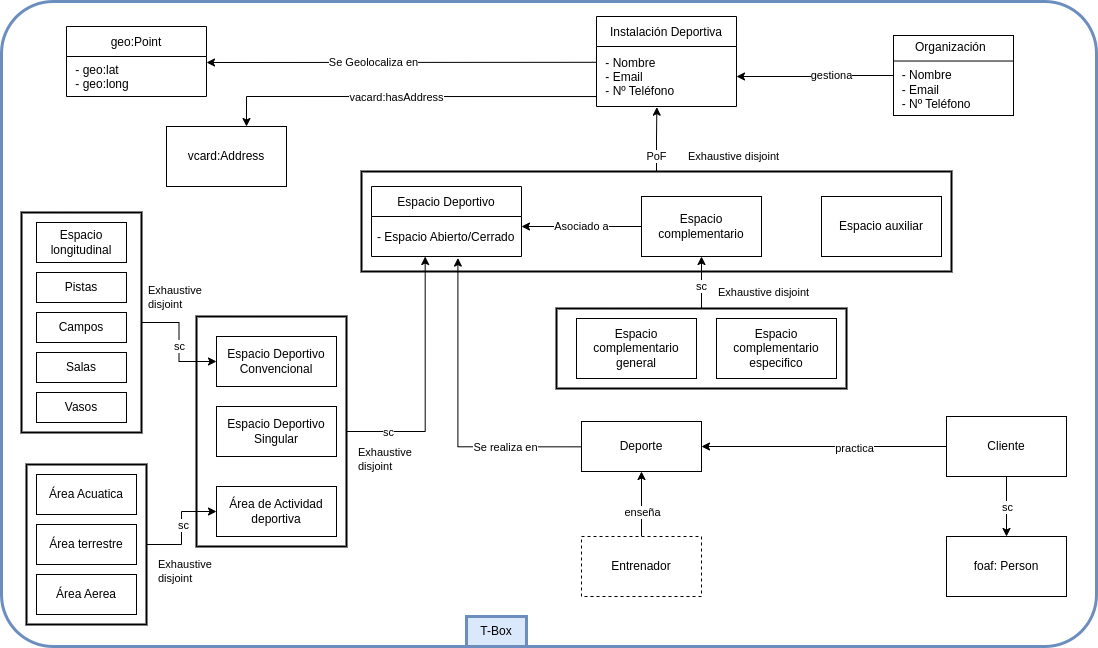
\includegraphics[width=0.7\textwidth]{include/tbox.jpg}
		\caption{Sección correspondiente a los recursos no ontológicos en la ontología.}
	\end{figure}
	
	Es importante señalar que la estructura taxonómica del documento descrito exige desambiguar entre las relaciones "sub-clase de" (\textit{sc} en el diagrama) y "parte de" (\textit{PoF} en el diagrama).
	
	\section{Patrones en la ontología}
	% Search for some ontology design patterns in the ontology design pattern portal that could be reused in your development.
	
	Al diseñar esta ontología, vimos que algunos de los patrones de diseño ya existentes eran aplicables a nuestro caso de instalaciones deportivas. Concretamente, los patrones reutilizados han sido el de servicios ofrecidos y el de normas.
	
	Para el diseño de los servicios ofrecidos por la organización en una instalación deportiva, se reutilizó el patrón de una relación N-aria según lo visto en clase. Este patrón se utiliza para representar una relación N-aria en el que todos los elementos tienen la misma importancia. Para representar esta relación N-aria se crea una clase, en nuestra ontología la clase \textit{ServicioOfrecido}, a la que asociar todos los atributos de la relación. Este patrón se utilizará para representar los servicios que una organización ofrece que se realizaran en una instalación deportiva en un horario determinado y por un precio indicado.
	
	\begin{figure}[H]
		\centering
		\includegraphics[width=0.6\textwidth]{include/patron_servicios.png}
		\caption{Esquema del patrón de servicios.}
	\end{figure}

	El patrón de normas está destinado a la definición de una serie de reglas y normas que aplican a la organización. Este patrón se representa utilizando la ontología \textbf{odrl}, y se define mediante la estructura: “Una \textit{acción} es \textit{permitida/obligatoria/prohibida} de ser realizada por una \textit{parte} sobre el \textit{activo}, siempre que se mantengan las \textit{restricciones}”.
	
	\begin{figure}[H]
		\centering
		\includegraphics[width=0.5\textwidth]{include/patron_reglas.png}
		\caption{Esquema del patrón de servicios.}
	\end{figure}
	
	En la sección de modelado conceptual de la ontología se entrará más en detalle sobre las clases y relaciones de estos patrones.
	
	\section{Modelo conceptual}
	% Build a conceptual model that integrates outcomes from the previous sections (c,d,e). This is the most important part of the work you are doing. Try to use:
	%  	i. Top level ontologies and other well-known ontologies. Classify in the pyramid of ontologies (figure use vs reuse) each of the ontologies that you reuse.
	%   ii. Transform each non-ontology resource into an ontology by using the T-box, A-Box or Population.
	%   iii. Select some Ontology Design Patterns (events, sequence, etc.)
	%   iv. Build the conceptual model of your ontology by integrating the above sources. The conceptual model should have at least 40 concepts, several subclass-of relations, disjoint, part-of (if needed), and ad-hoc relations.
	
	Tras el proceso de búsqueda de recursos ontológicos y no ontológicos para su reutilización como se ha explicado en los apartados anteriores, así como la selección de patrones de diseño de ontologías, se desarrolló el modelo conceptual de esta ontología. 
	
	Esta es una de las fases más importantes en la construcción de ontologías y en este apartado se describirán las clases y relaciones que se han implementado, y que en los siguientes apartados se formalizarán a código OWL. Debido al tamaño del modelo y para un mejor entendimiento se procederá a explicar los distintos módulos del modelo por separado. El diagrama completo de la ontología está disponible en el anexo.
	
	Encontramos cuatro clases principales que serán el núcleo de esta ontología. Estas clases son \textbf{Organización}, \textbf{Instalación Deportiva}, \textbf{Servicio Ofrecido} y \textbf{Regla}.
	
	
	\subsection{Organización}
	
	En lo que a la organización respecta, reutilizando clases y relaciones de la ontología \textbf{org} hemos creado el modelo que se puede observar en la figura a continuación. La forma de interpretar esta parte del modelo es: “Una organización encargada de gestionar instalaciones deportivas establece acuerdos de membresía con sus trabajadores para que estos tengan un determinado rol dentro de la organización”. Analizando el modelo con sus clases y relaciones tenemos:
	
	\begin{itemize}
		\item Una organización es \textit{SubClassOf} de \textit{org:Organization}. Organización tiene como propiedades el \textit{Nombre}, \textit{Email} y \textit{Número de teléfono}, que son literales.
		\item Una organización es la que gestiona una o más instalaciones deportivas, por lo que la clase \textit{Instalación Deportiva} se relaciona con \textit{Organización} mediante la relación \textit{managedBy}.
		\item Una \textit{Organización} establece unos acuerdos de membresía con sus trabajadores para un determinado rol (tal y como está definido en la ontología \textbf{org}) por lo que tenemos la clase \textit{org:Membership} que se relaciona con \textit{Organización} mediante la relación \textit{org:organization}. Esta clase se relaciona con las clases de cada trabajador mediante la relación \textit{org:memberOf} y se relaciona con \textit{org:Role} mediante la relación \textit{org:role}.
		
		Al diseñar esta sección hemos querido contemplar la posibilidad de que un trabajador de la organización tenga asignada la instalación o las instalaciones en las que trabaja por lo que hemos unido \textit{org:Membership} con \textit{Instalación Deportiva} mediante la relación \textit{establecidaEn}.
		\item Para determinar los tipos de trabajadores que hay en una organización hemos decidido crear una clase para cada uno de los tipos. Debido a la gran cantidad de clases de trabajadores que existen, hemos indicado las clases Monitor, Limpiador y Entrenador como ejemplo, todas ellas \textit{SubClassOf} de \textit{foaf:Person}.
	\end{itemize}

	\begin{figure}[H]
		\centering
		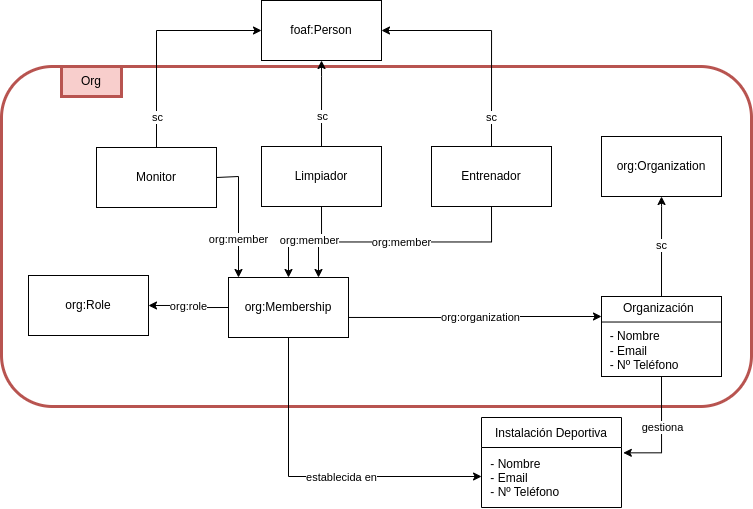
\includegraphics[width=\textwidth]{include/org.jpg}
		\caption{Esquema de las principales clases relacionadas con \textbf{Organización}.}
	\end{figure}
	
	\subsection{Instalación Deportiva}
	
	Para la construcción de la taxonomía de las instalaciones deportivas se ha hecho uso del recurso no ontológico explicado en apartados anteriores, y mediante un T-Box se ha modelado a nuestra ontología.
	
	\begin{itemize}
		\item Una Instalación Deportiva puede estar compuesta por diferentes elementos que forman parte de ella (\textit{partOf}): \textit{Espacio Deportivo} (que puede ser al aire libre o cerrado), \textit{Espacio Complementario} y \textit{Espacio Auxiliar}. Estas partes son disjuntas unas de otras. Según el documento de referencia, un \textit{Espacio Complementario} va asociado a un \textit{Espacio Deportivo}.
		\item Cada una de estas partes tiene su propia taxonomía tal y como se define en el recurso no ontológico y se muestra las diferentes subclases y las clases que son disjuntas (recuadros rosas) en el esquema de la Figura 8.
		\item La clase \textit{Instalación Deportiva} cuenta con propiedades como número\textit{ de teléfono} e \textit{email} que serán literales y no clases.
		\item Una instalación deportiva se geolocaliza en un \textit{geo:Point} mediante la relación \textit{hasGeopoint}. A su vez expresamos su localización mediante una dirección, para ello relacionamos \textit{Instalación Deportiva} con la clase \textit{vcard:Address} mediante la relación \textit{vcard:hasAddress}.
		\item La clase \textit{Deporte} se relaciona con un \textit{Espacio Deportivo} mediante la relación \textit{esPracticadoEn}.
		\item La clase \textit{Cliente} es \textit{subClassOf} \textit{foaf:Person}, y \textit{Cliente} practica uno o varios \textit{Deportes}. En el siguiente modulo también se verá que \textit{Cliente} consume un \textit{ServicioOfrecido}
		\item \textit{Entrenador} y \textit{Monitor} (definidos en el apartado de organización) tienen una relación con Deporte que es \textit{enseña}.
	\end{itemize}

	\begin{figure}[H]
		\centering
		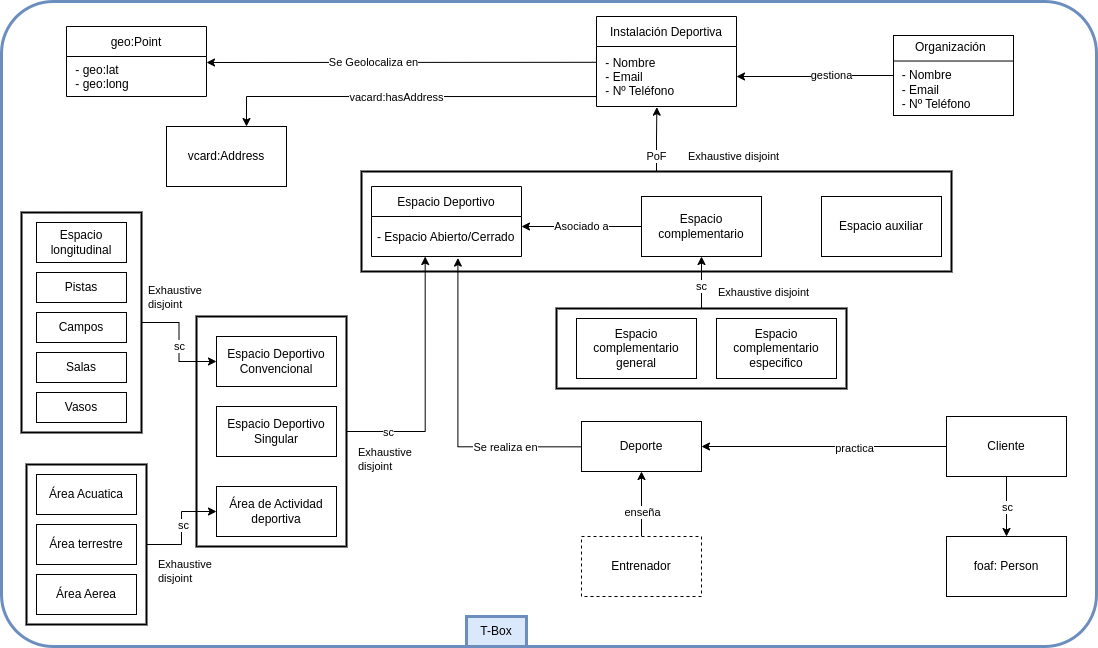
\includegraphics[width=\textwidth]{include/tbox.jpg}
		\caption{Esquema de las principales clases relacionadas con \textbf{Instalación Deportiva}.}
	\end{figure}
		
	\subsection{Servicio Ofrecido}
	
	La clase \textit{ServicioOfrecido} tiene asociadas varias clases mediante las relaciones indicadas.
	
	\begin{itemize}
		\item La clase \textit{Servicio}, que tiene dos subclases disjuntas \textit{Individual} y \textit{Bono de servicios}. De estas dos clases habría más subclases, para ejemplificar hemos incluido el alquiler de una pista de pádel o un bono de 10 clases de zumba.
		\item La clase \textit{Instalación Deportiva} en la que se ofrece el servicio. Por ejemplo, una pista de pádel, o la sala de musculación.
		\item \textit{time:DurationDescription} y \textit{time:GeneralDateTimeDescription}, que indicarán la duración y/o la fecha en la que se ofrece el servicio. Por ejemplo, "jueves 3 de noviembre del 2022 de 18:00 a 19:00", ó "todos los lunes y miércoles de febrero de 15:00 a 16:00".
		\item La clase \textit{PriceSpecification}, teniendo asociada como propiedades una cantidad y una moneda de pago. Por ejemplo 59,99 euros.
	\end{itemize}
	
	\begin{figure}[H]
		\centering
		\includegraphics[width=\textwidth]{include/pattern.jpg}
		\caption{Esquema de las principales clases relacionadas con \textbf{Servicio Ofrecido}.}
	\end{figure}
	
	\subsection{Regla}
	
	Al incluir este patrón de normas, hemos creado una única regla para ejemplificar las normas de
	una organización (en la realidad habría muchas de ellas, pero para simplificar el modelo para este trabajo se ha trabajado solo con una). Las reglas constan de la clase \textit{Rule} que define si se trata de una prohibición, una obligación o permiso, y de ella salen varias relaciones a una serie de clases que serán \textit{subclass of} de las siguientes entidades de la ontología \textbf{odrl}:
	
	\begin{itemize}
		\item \textbf{odrl:Constraint}. Para cada norma hay una \textit{subclass} de \textit{odrl:Constraint} y puede ser un lugar físico (piscina, pista de tenis, gimnasio) o un marco temporal (los sábados, el día 1 de cada mes, todos los días de 9:00 a 10:00) en el que se aplica la norma.
		\item \textbf{odrl:Asset}. Para cada norma tendremos una clase \textit{subclass of} \textit{odrl:Asset} que establece el activo o recurso que es sujeto de la norma. Este activo puede ser cualquier forma de recurso identificable, como datos/información, servicios o elementos físicos. En nuestra ontología hemos puesto el ejemplo de gorro de baño.
		\item \textbf{odrl:Action}. Para cada norma tendremos una clase \textit{subclass of} \textit{odrl:Action} que indicará la acción realizada sobre el activo. En nuestro modelo encontramos la clase Llevar puesto para el caso de gorro de baño.
		\item \textbf{odrl:Party}. Tendremos una \textit{subclass} de esta clase de odrl para cada regla, y definirá a qué parte de las personas se le aplica dicha regla. Puede ser por ejemplo una regla que aplique a todos los usuarios, o una regla que aplique sólo a trabajadores.
	\end{itemize}
	
	\begin{figure}[H]
		\centering
		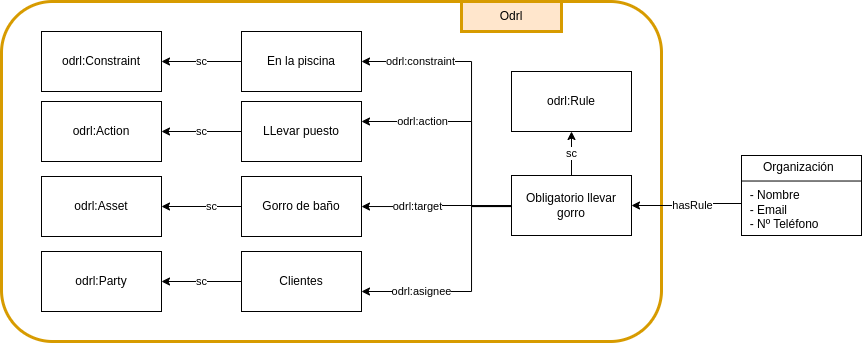
\includegraphics[width=\textwidth]{include/reglas.jpg}
		\caption{Esquema de las principales clases relacionadas con \textbf{Regla}.}
	\end{figure}
	
	\section{Implementación de la ontología con OWL}
	% Implement the ontology in an ontology development tool, or other ontology editor, using OWL as ontology language
	
	Como se ha especificado en los requisitos, la ontología será implementada en OWL, utilizando el programa Protégé, un editor de ontologías open source.
	
	El primer paso fue incluir todas las clases de la ontología creadas mediante el T-Box.
	
	Después, se crearon las clases obtenidas de la reutilización de las ontologías nombradas en el apartado 5. Para ello, se importaron las ontologías con su URI y se movieron los axiomas necesarios a nuestra ontología. En general, la metodología para importar las ontologías fue idéntica para todas: primero importar la ontología al completo con su URI, moviendo los axiomas necesarios, y después eliminar el resto. La única excepción fue la ontología \textbf{time}. Esta fue importada al completo, ya que utilizábamos la totalidad de sus entidades. Nos hemos dado cuenta al importar la ontología, que muchas de las propiedades estaban incompletas: les faltaba el rango o el dominio. Hemos optado por mantenerla como estaba, ya que muchos de estos problemas se debían a términos deprecados, y no hemos encontrado una versión más reciente de la ontología. 
	
	Una vez importadas las clases reutilizadas, definimos aquellas clases necesarias para completar nuestro modelo, que no se encontraban ni en el T-Box ni en las ontologías de alto nivel, como por ejemplo la clase Monitor, Entrenador, Pista de Baloncesto, etc.\\
		
	Este mismo procedimiento se realizó para los Object Properties. En este caso, además de importar los Object Porperties de las diferentes ontologías y crear los que necesarios no incluidos, definimos las propiedades de cada propiedad.
		
	Tuvimos cierta dificultad a la hora de crear la propiedad \textit{part of}, ya que tiene varios dominios para un único rango (tanto los espacios deportivos, como los complementarios y auxiliares son \textit{part of} una instalación deportiva), pero es una relación tradicionalmente transitiva. Para evitar problemas, decidimos que no fuese una relación transitiva.\\
		
	De forma similar, añadimos los Data Properties. En lugar de apuntar a una entidad, estas propiedades apuntan a un literal, por lo que hemos tenido que especificar los tipos de datos para literales como la divisa, el precio, etc. Un caso particular ha sido la propiedad \textit{hasCeiling} (tiene techo), para definir los Espacios Deportivos. En este caso el literal era un booleano.\\
	
	Finalmente, se completaron las labels y comentarios de aquellas entidades que no fueron directamente importadas, asegurando que estaban disponibles tanto en inglés como español. 
	
	En el anexo se puede encontrar una imagen de la jerarquía de las clases, los Object Properties y los Data Properties presentes en la ontología.
	
	Una vez finalizada la implementación de la ontología, se exportó como RDF para poder evaluarla con OOPS!
	
	\section{Evaluación de la ontología con OOPS!}
	% Evaluate the ontology with OOPS! and include in your report the pitfalls found. It is highly advisable to combine this evaluation with other ontology evaluation techniques.
	% Improve your ontology (conceptual model and implementation) taking into account the suggestions given by OOPS!. Iterate in these steps until the ontology pass most of the OOPS! recommedations.
	La ontología diseñada se ha evaluado utilizando la herramienta OntOlogy Pitfall Scanner! (OOPS!)\cite{oops}, que identifica errores en la ontología dividiéndolos en críticos, importantes y menores, de acuerdo a una batería errores comunes.
	
	\subsection{Mejoras implementadas tras la sugerencia de OOPS!}
	
	Tras la primera iteración de la evaluación con OOPS!, la herramienta destacó los siguientes problemas críticos:
	
	\begin{itemize}
		\item \textbf{P19:} Propiedades con múltiples rangos o dominios.
		
		Una de las relaciones definidas tenía más de un dominio, habiendo escrito en  accidentalmente \textit{and} en lugar de \textit{or} en el dominio.
		
		Los dominios de las relaciones \textit{time:hasDateTimeDescription} y \textit{time:hasTemporalDuration} fueron modificados añadiendo una entrada en sus dominios y eliminando la entrada de la ontología time. Esta modificación no fue aplicada por Protégé, y hubo que modificar la entrada del dominio impuesta por importar la ontología time para que el cambio quedase registrado.
		
		\item \textbf{P29:} Relaciones transitivas mal definidas.
		
		Las relaciones \textit{partOf}, \textit{hasService}, \textit{managed\_by} y \textit{constraint} estaban definidas como transitivas, teniendo rangos y dominios distintos. Por definición una propiedad transitiva debe tener el mismo rango y dominio.
		
		En el caso de \textit{partOf}, una relación que generalmente es transitiva, decidimos eliminar esta propiedad, ya que para nuestro modelo aparece únicamente entre Instalación Deportiva y los espacios deportivos, complementarios y auxiliares, que nunca serán unos parte de otros.
		
		Las otras relaciones se encontraban en esta clasificación por un error en la transcripción a Protégé.
	\end{itemize}
	
	Las propiedades \textit{vcard:hasEmail} y \textit{vcard:hasTelephone} aparecen como propiedades sin rango (P11), marcado como error importante, por ser su rango una clase deprecada de la ontología vcard. Pese a estar deprecada, esto no es un error, por lo que no se solucionó el problema.
	
	Gracias a las indicaciones de OOPS!, se pudo solucionar todos los errores críticos y varios otros clasificados como importantes. Se decidió no solucionar los errores no críticos de las ontologías importadas debido a las restricciones temporales sobre la entrega del trabajo y a la prioridad que se impuso sobre la reutilización de esta ontología.
	
	\subsection{Resultados finales de la evaluación}
	
	Tras aplicar las correcciones sobre los errores críticos indicados por OOPS! la última versión de la ontología tiene $11$ errores importantes, $63$ errores menores y $16$ sugerencias, mientras que en su primera iteración tenía $8$ errores críticos, $12$ errores importantes y $70$ errores menores, así como $16$ sugerencias.
	
	Cabe destacar que aproximadamente el $40\%$ de los errores indicados originalmente por OOPS! estaban relacionados con la ontología importada \textbf{time}.
	
	Los resultados completos de ambas evaluaciones se pueden encontrar en el Anexo.
	
	\section{Documentación de la ontología}
	% Document the ontology with Widoco and use Ontoology if required
	La documentación de la ontología fue generada utilizando la herramienta WIDOCO \cite{widoco}. Esta documentación está en un formato html, adjunto junto con este fichero, y su impresión en pdf también se encuentra adjunta.
	%\includepdf[pages=-]{include/documentation-widoco.pdf}
	
	\section{Conclusiones}
	Durante el proceso de creación de esta ontología, hemos podido aprender y tocar diversas
áreas de la ingeniería ontológica, nos hemos enfrentado a procesos de búsqueda y
planteamiento conceptual para la satisfacción de los requisitos planteados, y hemos tenido que
resolver los problemas que iban surgiendo en las distintas etapas.
	
	Después de completar todas las secciones del trabajo y a modo de conclusión, nos gustaría
	recapitular los conceptos y actividades relacionadas con el creación de ontologías que hemos
	aprendido a lo largo del desarrollo de este trabajo:
	\begin{itemize}
		\item Seguimiento de la metodología NeOn para el desarrollo de ontologías.
		\item Planteamiento de requisitos necesarios para nuestra ontología.
		\item Búsqueda y selección de los recursos ontológicos para su posterior reutilización, ya sea
de ontologías enteras o extracción de módulos de estas.
		\item Búsqueda de recursos no ontológicos para su posterior introducción en el modelo
		conceptual mediante T-box.
		\item Reutilización de patrones de diseño de ontologías, concretamente los patrones de
		servicio y normas.
		\item Modelado conceptual de la ontología con todos los elementos anteriores e
		introduciendo clases y relaciones necesarias para completarlo y cubrir los requisitos.
		\item Implementación y formalización en OWL con la herramienta Protege.
		\item Evaluación de la ontología creada gracias al uso de herramientas como OOPS! para su
		posterior corrección.
		\item Documentación de la ontología gracias a WIDOCO.
	\end{itemize}
	En definitiva, ha sido un trabajo que ha involucrado muchas áreas diferentes sirviendo así como
introducción al complejo mundo de las ontologías.
	
\newpage
	\section*{Bibliografía}
	\addcontentsline{toc}{section}{Bibliografía}
	\bibliography{include/references}
	\bibliographystyle{IEEEtran}
	
	\newpage
	\section*{Anexos}
	\addcontentsline{toc}{section}{Anexos}
	
	\begin{figure}[H]
		\centering
		\includegraphics[height=\textheight]{include/classes.png}
		\caption{Jerarquía de clases de la ontología.}
	\end{figure}

	\begin{figure}[H]
		\centering
		\includegraphics[width=\textwidth]{include/object.png}
		\caption{Object Properties presentes en la ontología.}
	\end{figure}
	
	\begin{figure}[H]
		\centering
		\includegraphics[width=\textwidth]{include/data.png}
		\caption{Data Properties presentes en la ontología.}
	\end{figure}
	
		\begin{figure}[H]
		\centering
		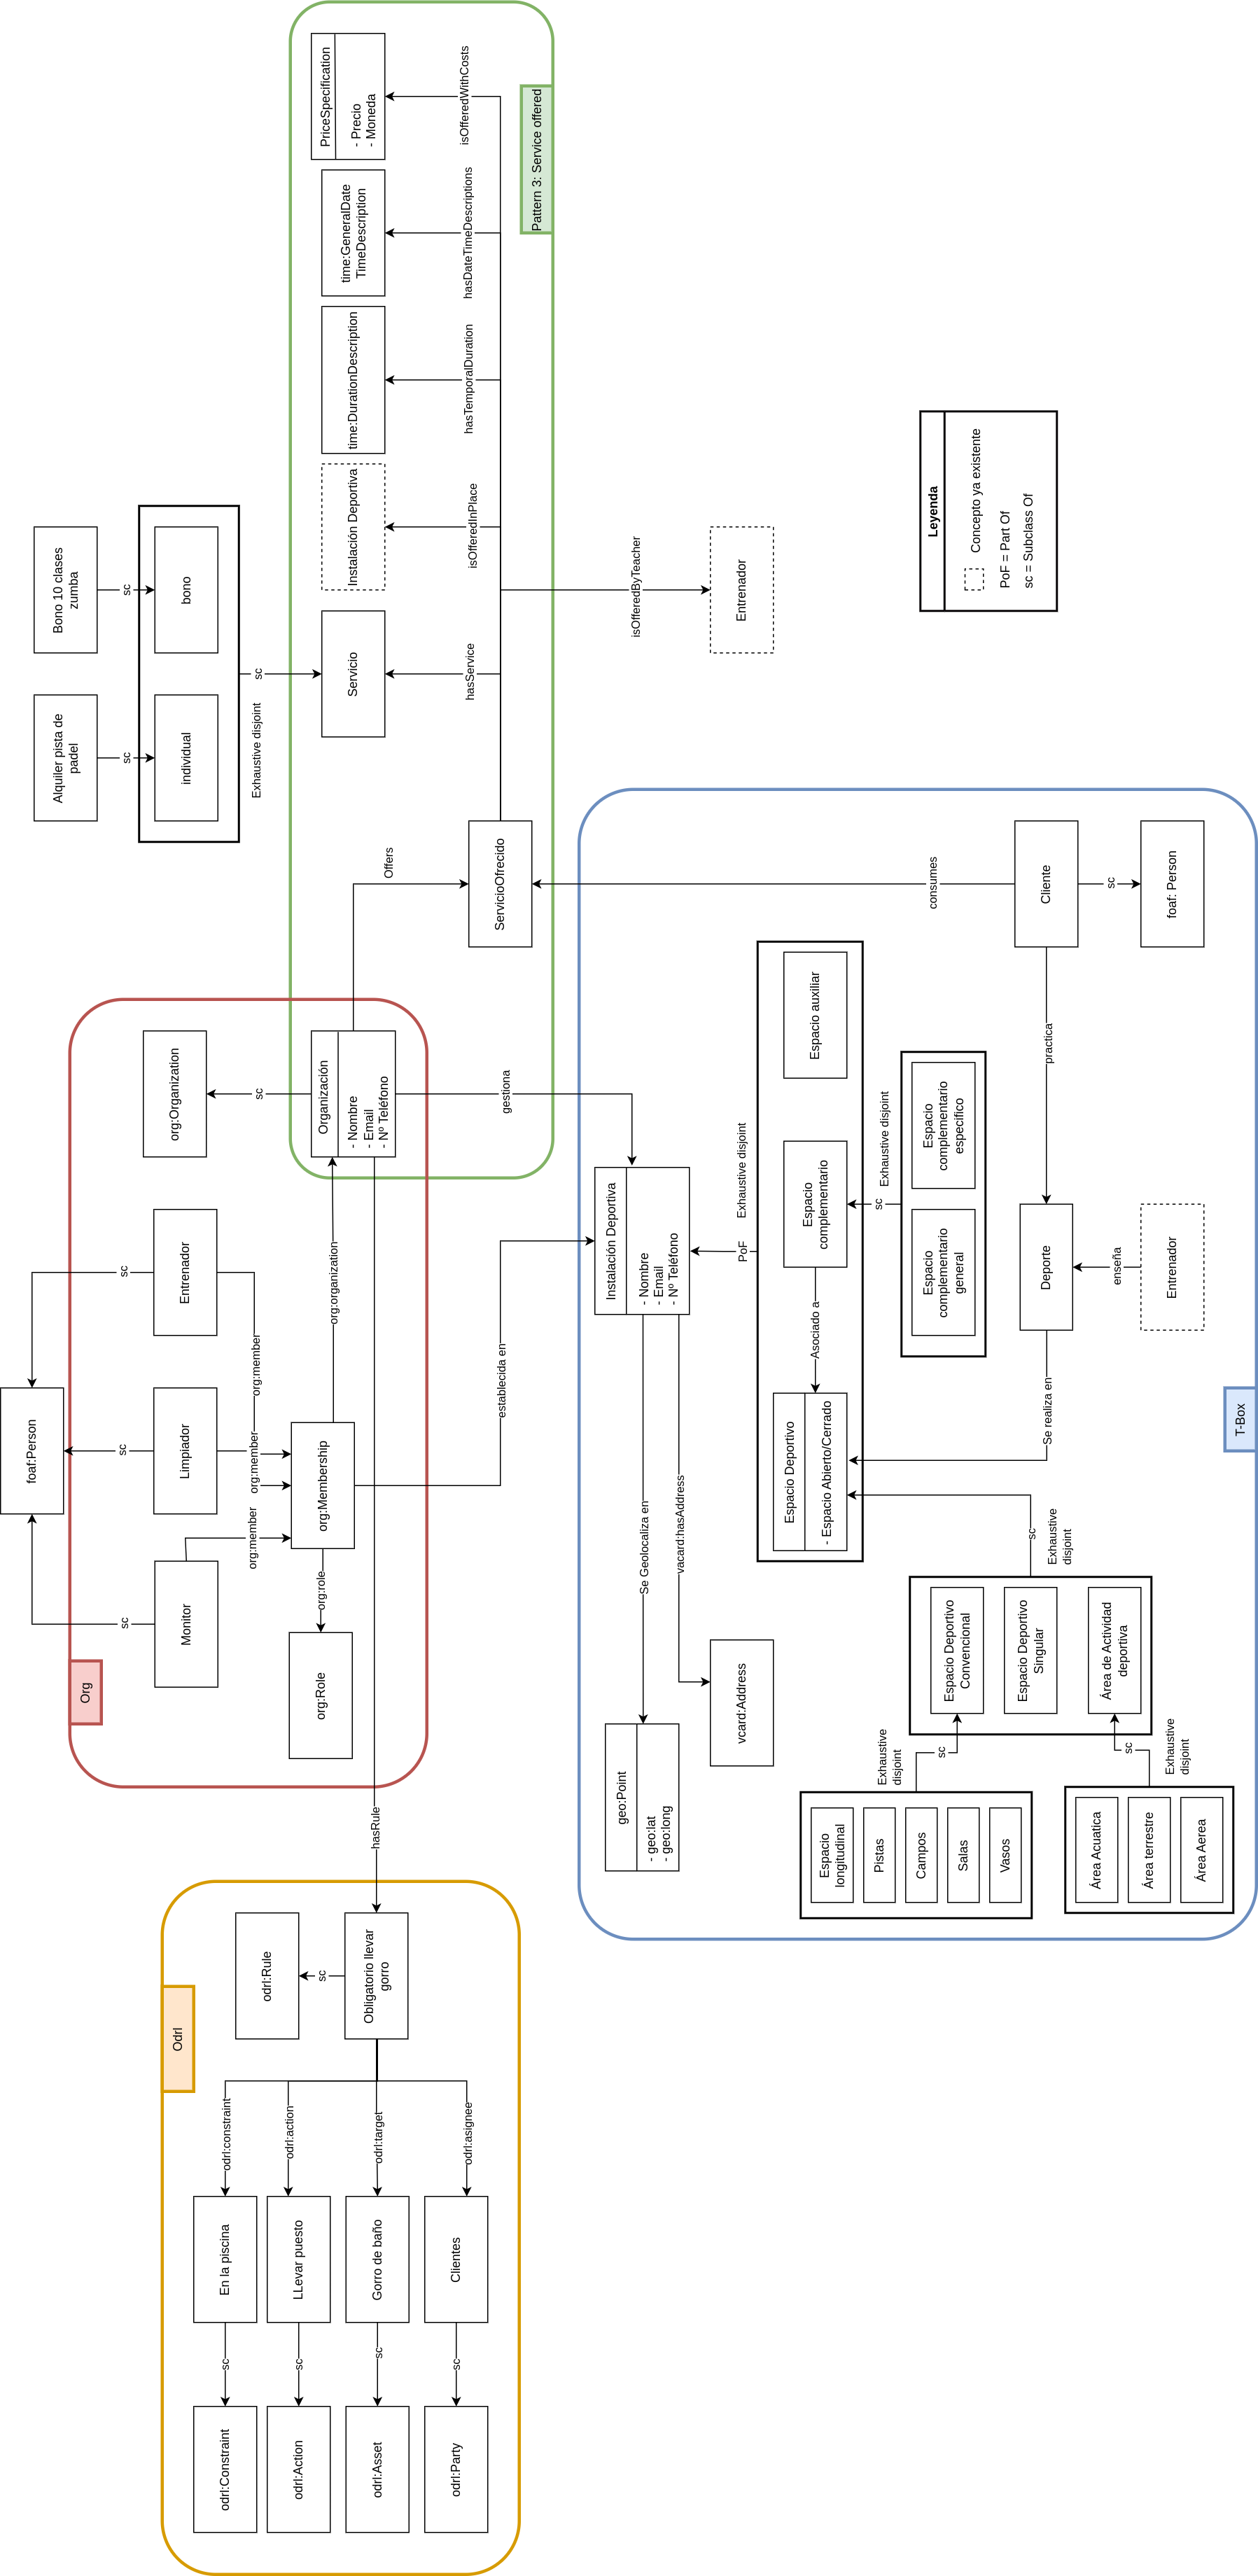
\includegraphics[width=0.85\textwidth]{include/diagrama_modelo_completo.png}
		\caption{Diagrama completo del modelado de la ontología.}
	\end{figure}
	
	\begin{figure}[H]
		\begin{subfigure}{.5\textwidth}
			\centering
			\includegraphics[height=\textheight]{include/eval_inicial_oops.png}
			\caption{Resultados iniciales de la evaluación con OOPS! }
		\end{subfigure}
		\begin{subfigure}{.5\textwidth}
			\centering
			\includegraphics[height=\textheight]{include/eval_final_oops.png}
			\caption{Resultados finales de la evaluación con OOPS!}
		\end{subfigure}
		\caption{Diferentes resultados obtenidos de la evaluación con OOPS!}
	\end{figure}
	
	%\subsection*{Documentación (español)}
	%\includepdf[pages=-]{include/documentacion-es.pdf}
	%\input{./include/portada.tex}
	


\end{document}